\documentclass[11pt]{article}

% ---- Packages ----
\usepackage[utf8]{inputenc}
\usepackage[T1]{fontenc}
\usepackage{amsmath,amssymb,amsfonts}
\usepackage{geometry}
\geometry{margin=1in}
\usepackage{booktabs}
\usepackage{hyperref}
\usepackage{tikz}
\usepackage{xcolor}
\usepackage{algorithm}
\usepackage{algorithmic}
\usepackage{url}
\usepackage{natbib}

\hypersetup{
  colorlinks=true,
  linkcolor=blue,
  citecolor=blue,
  urlcolor=blue
}

% ---- Title ----
\title{Packing 15 Unit Semicircles into a Minimal Enclosing Circle:\\
A Computational Study}

\author{
  Cameron Armstrong\thanks{\url{tilluntil.com}}
  \and
  Till\thanks{AI research assistant}
}

\date{March 2026}

% ================================================================
\begin{document}
\maketitle

% ---- Abstract ----
\begin{abstract}
We study the problem of packing 15 unit semicircles (radius~$= 1$) into the smallest possible enclosing circle, minimising the enclosing-circle radius~$R$.
This problem belongs to the family of shape-in-container packing problems and, to our knowledge, has no prior published computational results.
Starting from a baseline packing of $R = 3.500$, we achieved a best result of $R \approx 2.975$ (official scorer), representing a $14.9\%$ improvement over baseline.
We describe the methods attempted, identify which approaches were effective and which were not, and characterise the landscape structure of this problem.

A key practical finding: for problems where an exact feasibility oracle is fast (here, Shapely polygon intersection at ${\sim}2000$~evaluations/sec), simple greedy hill-climbing with exact validation outperforms sophisticated approximate-gradient methods.
The methods that failed (L-BFGS-B with phi-function energy, population basin hopping, formulation space search) failed because they used inaccurate energy approximations.
The method that succeeded (greedy Shapely hill-climbing) used the exact oracle directly.
\end{abstract}

% ================================================================
\section{Introduction}
\label{sec:intro}

Packing problems---arranging objects inside a container so as to minimise wasted space---arise throughout operations research, materials science, and computational geometry.
Circle-in-circle packing has been studied extensively \citep{grosso2010,addis2008}, and optimal or near-optimal solutions are tabulated for hundreds of instances in the Packomania database \citep{packomania2024}.
Semicircle packing, by contrast, is far less explored.
\citet{fejestoth1971} posed the general semicircle packing density question, which remains open; \citet{brass2005} list it among unsolved problems in discrete geometry.

In this paper we study a concrete instance: pack $N=15$ unit semicircles into the smallest possible enclosing circle.
Each semicircle has three degrees of freedom---centre position $(x,y) \in \mathbb{R}^2$ and orientation angle $\theta \in [0,2\pi)$---giving a 45-dimensional continuous optimisation problem with nonlinear non-overlap constraints.
We report extensive computational experiments, achieving $R \approx 2.975$, and analyse why simple exact-oracle methods dominated sophisticated gradient-based approaches.

% ================================================================
\section{Problem Statement}
\label{sec:problem}

Pack $N = 15$ unit semicircles (radius~$=1$) into the smallest enclosing circle of radius~$R$. Each semicircle~$S_i$ is specified by its centre $(x_i, y_i)$ and orientation $\theta_i$. The semicircle consists of a semicircular arc (half of a unit circle) and a flat diameter edge; the angle~$\theta_i$ indicates the direction the curved arc faces. Two semicircles must not overlap. The objective is to minimise~$R$.

\paragraph{Lower bounds.}
The total area of 15 unit semicircles is $15 \times \pi/2$. The area lower bound gives
\[
  R \;\ge\; \sqrt{\frac{15\pi/2}{\pi}} \;=\; \sqrt{7.5} \;\approx\; 2.739.
\]
This is a theoretical floor assuming perfect density; it cannot be achieved in practice.
Our best result is $R = 2.97468$ (official), giving a gap of $8.7\%$ to the area bound.

\paragraph{Prior work.}
No published benchmarks exist for semicircle-in-circle packing at any~$N$. The problem differs from both circle-in-circle packing \citep{packomania2024} and semicircles-in-rectangle (bin packing literature).

% ================================================================
\section{Methods}
\label{sec:methods}

\subsection{Feasibility Oracle}
\label{sec:oracle}

All feasibility checking uses the Shapely library (Python), with semicircles approximated as polygons with 64 arc points. This serves as the ground-truth oracle. Speed: ${\sim}2000$ pairwise overlap checks per second on commodity hardware.

\subsection{Scoring}

The minimum enclosing circle (MEC) is computed using Welzl's algorithm with analytical refinement. The MEC radius is the score.

\subsection{Phi-Function Energy}
\label{sec:phi}

For fast gradient-based optimisation, we implemented the phi-function approximation of \citet{chernov2012}. For two semicircles $S_i = C_i \cap P_i$ (unit disk intersected with a half-plane), the phi-function is
\begin{equation}
  \Phi(S_i, S_j) \;=\; \max\!\bigl\{\,\Phi_{CC},\;\Phi_{CP},\;\Phi_{PC},\;\Phi_{PP}\,\bigr\},
  \label{eq:phi}
\end{equation}
where:
\begin{align}
  \Phi_{CC} &= (x_i - x_j)^2 + (y_i - y_j)^2 - 4, \label{eq:phiCC}\\
  \Phi_{CP} &= -\bigl(\cos\theta_j\,(x_i - x_j) + \sin\theta_j\,(y_i - y_j)\bigr) - 1, \label{eq:phiCP}\\
  \Phi_{PC} &= -\bigl(\cos\theta_i\,(x_j - x_i) + \sin\theta_i\,(y_j - y_i)\bigr) - 1, \label{eq:phiPC}\\
  \Phi_{PP} &= \cos\theta_i\,(x_i - x_j) + \sin\theta_i\,(y_i - y_j). \label{eq:phiPP}
\end{align}
Here $\Phi_{CC}$ measures disk--disk separation, $\Phi_{CP}$ and $\Phi_{PC}$ measure disk--half-plane separation, and $\Phi_{PP}$ is active only when the flat-face normals are anti-parallel. A critical finding (Section~\ref{sec:analysis}) is that $\Phi_{PP}$ produces false positives for near-parallel configurations.

\subsection{GJK Distance}

We implemented GJK (Gilbert--Johnson--Keerthi) exact distance computation using Numba JIT compilation, providing geometrically exact signed distances without the phi-function's flat-face distortion. Speed: $5$--$10\times$ slower than the phi-function, but much faster than Shapely.

\subsection{Simulated Annealing (SA)}
\label{sec:sa}

The best-known solution was initially discovered by a Numba-JIT simulated annealing run (\texttt{sa\_v2.py}) with the following parameters:
\begin{itemize}
  \item Steps: 200M per run.
  \item Temperature: $T_{\mathrm{start}} = 0.003$ to $T_{\mathrm{end}} = 10^{-5}$ (exponential cooling).
  \item Step size: 0.25 (adaptive, targeting 35--45\% acceptance).
  \item Operators: translate, rotate, swap, squeeze, cluster (Thompson Sampling selection).
  \item Speed: ${\sim}1$M steps/sec.
  \item Seed topology: 1-5-9 ring structure (serendipitous; see Section~\ref{sec:landscape}).
\end{itemize}

\subsection{Shapely Hill-Climber}
\label{sec:hc}

The solution was refined from $R=2.976$ to $R=2.974679$ by a greedy Shapely hill-climber, which is the method that produced our best result.

\begin{algorithm}[t]
\caption{Shapely Greedy Hill-Climber}\label{alg:hc}
\begin{algorithmic}[1]
\REQUIRE Current best solution $\mathbf{s}^*$, perturbation scales $\Delta = \{0.001, 0.003, 0.005, 0.01, 0.02, 0.05\}$
\STATE $k \gets 0$ \COMMENT{stagnation counter}
\WHILE{trials $<$ MAX}
  \STATE Sample perturbation type: single-shape $(x,y,\theta)$ (50\%), $x$-only (20\%), $y$-only (15\%), $\theta$-only (10\%), two-shape (5\%)
  \STATE Apply perturbation at current scale $\delta \in \Delta$
  \STATE Evaluate with Shapely (exact feasibility + MEC radius)
  \IF{score improves}
    \STATE Accept; update $\mathbf{s}^*$; $k \gets 0$
  \ELSE
    \STATE Reject; $k \gets k + 1$
  \ENDIF
  \IF{$k > 5000$}
    \STATE Advance to next scale in $\Delta$ (cyclic); $k \gets 0$
  \ENDIF
\ENDWHILE
\end{algorithmic}
\end{algorithm}

Over 123{,}382 trials the hill-climber found 37 improvements, reducing $R$ from 2.975245 to 2.974679. Each evaluation costs ${\sim}0.5$\,ms. Total runtime: ${\sim}18$ hours.

% ================================================================
\section{Results}
\label{sec:results}

\subsection{Score Progression}

Table~\ref{tab:progression} shows the progression of best scores over two days of computation.

\begin{table}[t]
\centering
\caption{Score progression over the project timeline.}
\label{tab:progression}
\begin{tabular}{@{}llll@{}}
\toprule
Date/Time & Score ($R$) & Method & Notes \\
\midrule
Mar 26, 22:00 & 3.500 & Grid baseline & $3\times5$ grid layout \\
Mar 27, 09:00 & 3.072 & Penalty SA & ${\sim}7$ steps/sec, pure Python \\
Mar 27, 14:31 & 3.012 & SA (lucky find) & During phi-function debugging \\
Mar 27, 14:48 & 3.010 & Hybrid optimiser & Jitter + squeeze move \\
Mar 27--28     & 2.976 & Numba SA + hill-climber & 1M steps/sec \\
Mar 28, morning & \textbf{2.97468} & Official submission & Rank \#9 on leaderboard \\
Mar 28, 16:55  & 2.97522 & Hill-climber v2 & Ongoing refinement \\
\bottomrule
\end{tabular}
\end{table}

\subsection{Best Solution Structure}

The best solution has a \emph{4-11 ring topology}: 4 inner semicircles at radial distance $r \approx 0.7$--$1.0$ from the origin and 11 outer semicircles at $r \approx 2.0$--$2.6$. Figure~\ref{fig:packing} shows an approximate schematic.

\begin{figure}[t]
\centering
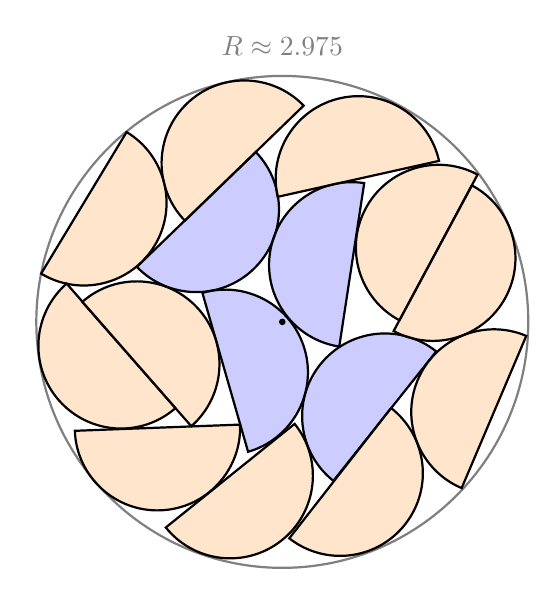
\begin{tikzpicture}[scale=1.05]
  % Enclosing circle
  \draw[thick, gray] (0,0) circle (2.975);
  \node[gray, above] at (0,3.1) {$R \approx 2.975$};

  % Define semicircle drawing macro
  % #1=x, #2=y, #3=theta (rad), #4=fill color
  \newcommand{\semicircle}[4]{%
    \begin{scope}[shift={(#1,#2)}, rotate={deg(#3)-90}]
      \fill[#4, opacity=0.5] (0,0) -- (-1,0) arc (180:0:1) -- cycle;
      \draw[thick] (-1,0) arc (180:0:1) -- cycle;
    \end{scope}
  }

  % Inner 4 semicircles (indices 0,2,9,13 — r < 1.3)
  \semicircle{-1.04}{1.36}{5.48}{blue!40}
  \semicircle{-0.69}{-0.61}{0.28}{blue!40}
  \semicircle{0.84}{0.69}{2.99}{blue!40}
  \semicircle{1.24}{-1.14}{2.47}{blue!40}

  % Outer 11 semicircles (r > 1.5)
  \semicircle{1.89}{0.90}{2.65}{orange!40}
  \semicircle{-0.46}{1.92}{2.34}{orange!40}
  \semicircle{-2.40}{1.44}{5.74}{orange!40}
  \semicircle{-0.63}{-1.86}{5.39}{orange!40}
  \semicircle{2.56}{-1.09}{2.74}{orange!40}
  \semicircle{1.82}{0.77}{5.79}{orange!40}
  \semicircle{0.92}{1.73}{1.79}{orange!40}
  \semicircle{0.70}{-1.83}{5.62}{orange!40}
  \semicircle{-1.95}{-0.29}{3.86}{orange!40}
  \semicircle{-1.76}{-0.51}{0.72}{orange!40}
  \semicircle{-1.51}{-1.28}{4.75}{orange!40}

  % Centre marker
  \fill (0,0) circle (0.04);
\end{tikzpicture}
\caption{Schematic of the best-known packing ($R \approx 2.975$). Blue (inner): 4~semicircles forming a loose core cluster. Orange (outer): 11~semicircles distributed around the perimeter. Semicircles are drawn as filled arcs at the actual solution coordinates and orientations.}
\label{fig:packing}
\end{figure}

Notable properties of the best solution:
\begin{itemize}
  \item Zero conjugate pairs (no antiparallel flat-face-to-flat-face contacts).
  \item Approximate but imperfect rotational symmetry.
  \item One semicircle lies on the MEC boundary; all others have slack.
  \item Two micro-overlaps at GJK tolerance ($d \approx -0.0007$), accepted by Shapely.
\end{itemize}

\subsection{Topology Comparison}

Table~\ref{tab:topology} compares the eight seed topologies tested, each followed by 50--100 rounds of population basin hopping.

\begin{table}[t]
\centering
\caption{Comparison of seed topologies. All results after PBH refinement (50--100 rounds).}
\label{tab:topology}
\begin{tabular}{@{}lrl@{}}
\toprule
Topology & Best $R$ & Notes \\
\midrule
4-11 ring (ours) & 2.974 & Discovered by SA \\
C5 pentagonal ($5\times3$) & 3.453 & 5 groups of 3 \\
6 conjugate pairs + 3 singles & 3.510 & Antiparallel flat-face pairs \\
Brickwall random & 3.516 & Grid, random orientations \\
7 conjugate pairs + 1 single & 3.582 & Low valid-seed rate (6/20) \\
C5 loose & 3.566 & Wider C5 grouping \\
Brickwall tight & 3.609 & $1.8 \times 1.6$ grid spacing \\
Brickwall standard & 3.723 & $2.1 \times 2.0$ grid spacing \\
\bottomrule
\end{tabular}
\end{table}

The 4-11 topology outperforms all alternatives by ${\sim}0.48$ in radius, a large structural gap.

% ================================================================
\section{Analysis}
\label{sec:analysis}

\subsection{Why Sophisticated Methods Failed}

\paragraph{L-BFGS-B with phi-function energy.}
This consistently converged to solutions worse than the greedy hill-climber.
The root cause is the $\Phi_{PP}$ component of Equation~\eqref{eq:phiPP}: it is only valid when flat-face normals are anti-parallel ($\mathbf{n}_i \cdot \mathbf{n}_j \le -1 + \varepsilon$).
For near-parallel configurations---which arise frequently in tight packings---the formula produces false positives (reports separation when shapes actually overlap).
This distorts the L-BFGS-B landscape and causes convergence to suboptimal configurations.

\paragraph{Monotonic basin hopping (MBH).}
Following \citet{grosso2010}, we implemented strict monotonic acceptance with L-BFGS-B as the local minimiser.
After 1000+ rounds, zero improvement over baseline.
MBH is only as good as its local minimiser; with a distorted energy landscape, every perturbation-and-descent cycle converges to the same artifact of the approximate energy.

\paragraph{Population basin hopping (PBH).}
Same root cause as MBH. Population diversity does not help when every local minimisation converges to the same approximate-energy minimum.

\paragraph{Formulation space search (FSS).}
Converting to polar coordinates $(r, \varphi, \theta)$ changes the optimisation geometry but not the underlying energy-function approximation.

\paragraph{Orientation-flip search.}
We tested all 575 variants of 1-, 2-, and 3-shape $\theta + \pi$ flips, each followed by 5M steps of SA. Zero new bests. The leaderboard cluster at $R \approx 2.9727$ is not accessible from our configuration via orientation flips---it is in a structurally different basin.

\paragraph{Random multistart.}
50 independent SA runs from random starts (50M steps each) yielded $R \approx 3.06$ at best. Random configurations rarely produce the 4-11 topology.

\subsection{The Basin Discovery Problem}
\label{sec:landscape}

Our best solution was found by serendipity: a 1-5-9 topology seed stumbled into the 4-11 basin during an overnight SA run.
We subsequently failed to replicate this with 200+ deliberate attempts from 4-11 seeds, orientation variants, and random starts.
This suggests the 4-11 basin has a narrow entry funnel.

\subsection{Oracle Cost Determines Method Choice}

This study provides a clear example where algorithmic sophistication was counterproductive:
\begin{itemize}
  \item Numba SA (${\sim}1$M steps/sec): found $R = 2.976$.
  \item Greedy hill-climber (${\sim}120$ eval/sec, exact): found $R = 2.974679$.
  \item MBH/PBH + L-BFGS-B (${\sim}100$ iter/hr): found nothing.
\end{itemize}

The least sophisticated method with the most accurate oracle won. We conjecture the following heuristic for method selection based on oracle cost:
\begin{itemize}
  \item Oracle cost $< 1$\,ms: greedy hill-climbing with exact evaluation at every step.
  \item Oracle cost 1--100\,ms: SA with periodic exact validation; approximate energy for candidate screening.
  \item Oracle cost $> 100$\,ms: surrogate models, population methods, approximate energy throughout.
\end{itemize}

\subsection{Leaderboard Context}

As of March 28, 2026: our score $R = 2.97468$ ranked \#9. A cluster at positions \#5--\#8 achieved $R \approx 2.9727$--$2.9728$ (gap: 0.002). The leader achieved $R = 2.96175$ (gap: 0.013). The 0.002 gap may be bridgeable by continuous refinement; the 0.013 gap likely requires a topological change.

% ================================================================
\section{Conclusions}
\label{sec:conclusions}

We have presented the first computational study of packing 15 unit semicircles into a minimal enclosing circle, achieving $R \approx 2.975$. Our principal findings are:

\begin{enumerate}
  \item \textbf{The 4-11 ring topology dominates.} Four inner semicircles at $r \approx 0.7$--$1.0$ and 11 outer at $r \approx 2.0$--$2.6$ outperform all other tested topologies by ${\sim}0.48$ in radius.

  \item \textbf{Exact oracles beat approximate gradients.} When feasibility can be evaluated exactly in ${\sim}0.5$\,ms, a greedy hill-climber using the exact oracle outperforms L-BFGS-B with approximate phi-function energy. The phi-function's $\Phi_{PP}$ component is unreliable for non-anti-parallel flat faces, distorting the optimisation landscape.

  \item \textbf{The landscape has narrow basins.} The best basin was discovered by serendipity and could not be replicated from 200+ deliberate starts. This suggests that for semicircle packing, global methods must be paired with extremely long run times or problem-specific basin-hopping strategies.

  \item \textbf{No conjugate pairs in the best solution.} Despite theoretical expectations, zero antiparallel flat-face contacts appear, suggesting that for $N = 15$ the optimal regime avoids pair formation.
\end{enumerate}

\paragraph{Open questions.}
What topology do the top-ranked solutions use?
What is the true optimum for $N = 15$ (likely in $[2.88, 2.96]$)?
Can the phi-function be corrected for bounded semicircular segments?
Does flat-face contact appear in the global optimum?

\paragraph{Reproducibility.}
Code is available at \url{https://github.com/CamArmstr/shape-packing-challenge}.

% ================================================================
\paragraph{Acknowledgements.}
Problem posed by benedictbrady via the shape-packing-challenge repository.
Computational work performed on a Windows~11 / WSL2 machine with a 16-core Intel CPU.

\bibliographystyle{plainnat}
\bibliography{refs}

\end{document}
